\chapter{PROBLEMS}
% !TEX root = hazy2.tex

\section{Introduction}

The code is designed to be autonomous and self-aware.
Nonetheless, if can run into problems.
This section describes some of the errors that can cause
\Cloudy\ to stop.
Floating point errors should never occur.
Several other internal errors, which the code is designed to trap
and then complain about, could occur.
Finally, it is possible that the code will stop because of
convergence problems.

The most important single thing to understand about any calculation is
why it stopped and whether this affects the predictions.
This is discussed
further in the section \cdSectionTitle{Stopping Criteria}

If the calculation aborts it will conclude with a request to post the
information on the web site's discussion board---please do---we can't fix
it if we don't know it's broken.

Please post any problems on the discussion board on the code's
\href{https://cloudyastrophysics.groups.io}{discussion board}.

\section{Thermal stability and temperature convergence}
\label{sec:ThermalStabilityProblems}

This section describes thermal stability problems, how to identify them,
and what to do about them.

\subsection{Types of thermal maps}

Three types of thermal maps, showing the heating or cooling of gas as
a function of temperature, can be produced by \Cloudy.  Each is the answer
to a different question.

Figure \ref{fig:cooling_heating} shows the heating and cooling
rates as a function of temperature
for a photoionized gas in which the gas kinetic temperature was varied.
This figure was produced with the test case \cdFilename{func\_map.in},
one of the standard
test cases included in the code distribution.
Both the gas density and
the flux of ionizing photons were held constant and the kinetic temperature
was varied.
Only one temperature, the point where the two curves cross,
occurs in equilibrium.
The \cdFilename{func\_map.in} file uses the
\cdCommand{save map} command
to determine heating and cooling rates at a variety of temperatures.
This
is exactly what the code does to determine the equilibrium temperature,
so this plot can be useful to find out why the code ran into temperature
convergence problems.
This is why the command was introduced.

\begin{figure}
\centering
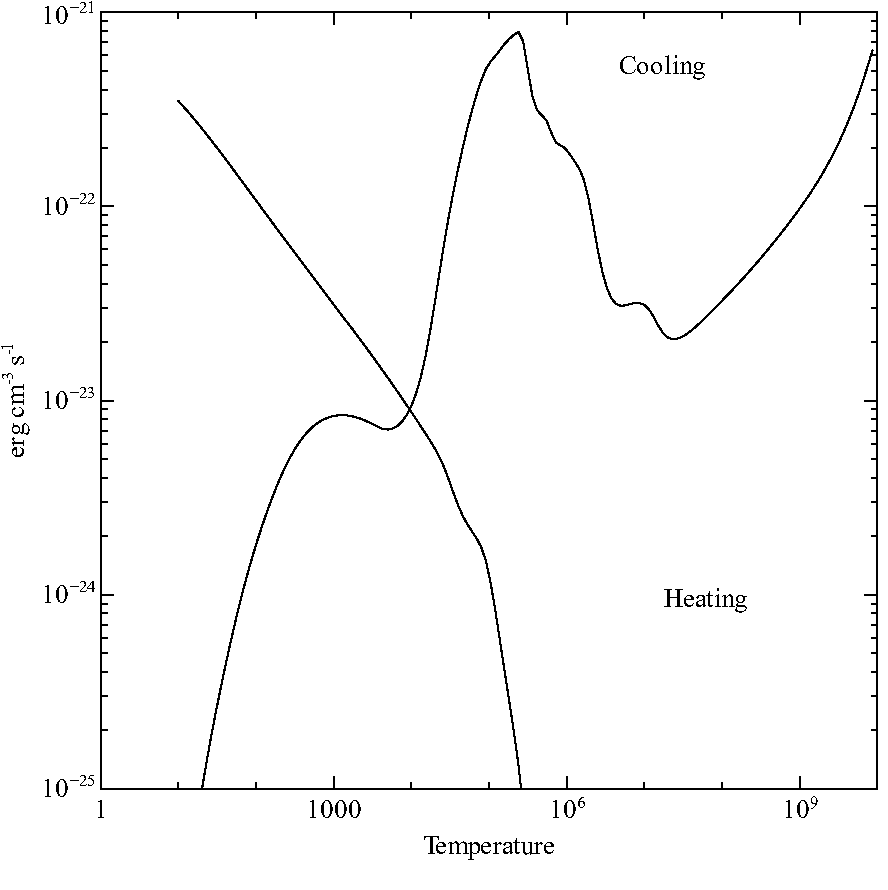
\includegraphics[scale=0.8]{cooling_heating}
\caption[Cooling and heating in a photoionized gas]{\label{fig:cooling_heating}A typical heating---cooling function for low density photoionized
gas. The cooling and heating rates (erg cm$^{-3}$ s$^{-1}$) are shown.  }
\end{figure}

Collisionally-ionized gas has a well-defined cooling rate that is only
a function of temperature.
The sample program
\cdFilename{hazy\_coolingcurve.cpp}
(included in the \cdFilename{programs} directory in the code's
distribution)  does such a
calculation, and Figure \ref{fig:coolcurve} shows the results.
Here the kinetic temperature
is set by some physics external to the calculation.
The entire ionization
solution is valid for each temperature under this assumption.
The
unspecified heat source would have to provide a local heating rate that
is equal to the calculated cooling rate for the solution to be time steady.

\begin{figure}
\centering
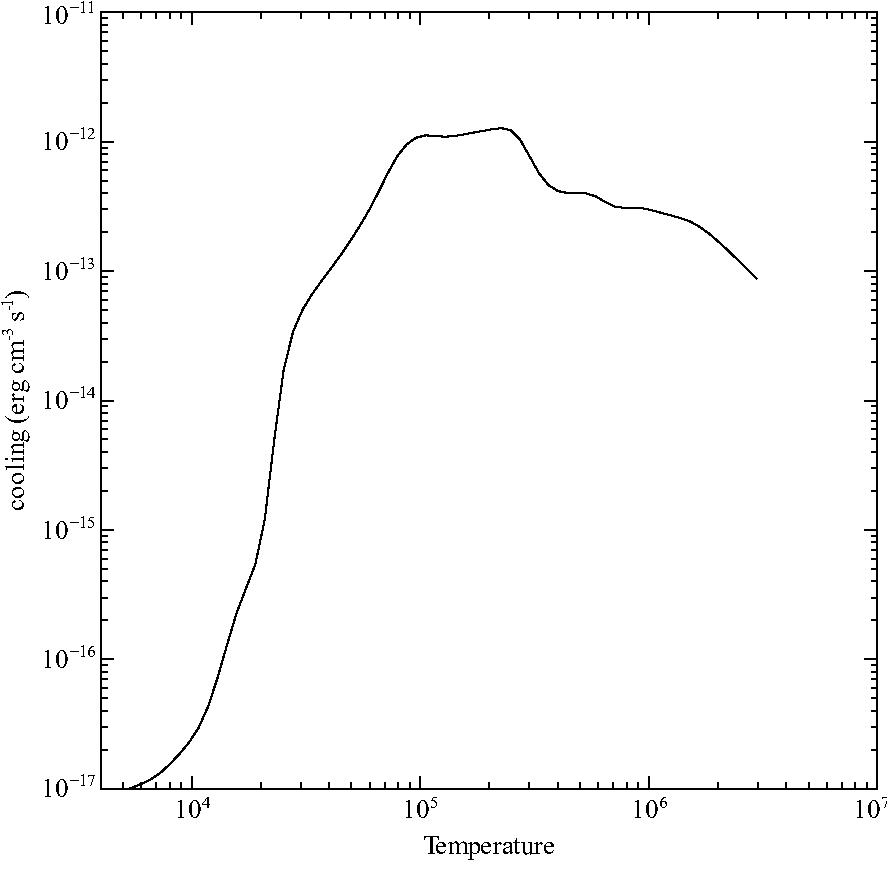
\includegraphics[scale=0.8]{coolcurve}
\caption[Cooling function for collisionally ionized gas]{\label{fig:coolcurve}A typical cooling function for low
density collisionally ionized gas.}
\end{figure}

The third map is the type of thermal stability map shown by \citet{Krolik1981} and plotted in Figure \ref{fig:hazy_kmt}.
The program that generated these
results is given in the file \cdFilename{hazy\_kmt.cpp}.
Here the equilibrium temperature
is determined self-consistently for gas over a wide range of densities,
but for a single flux of ionizing photons (or equivalently, distance from
the central object).

\begin{figure}
\centering
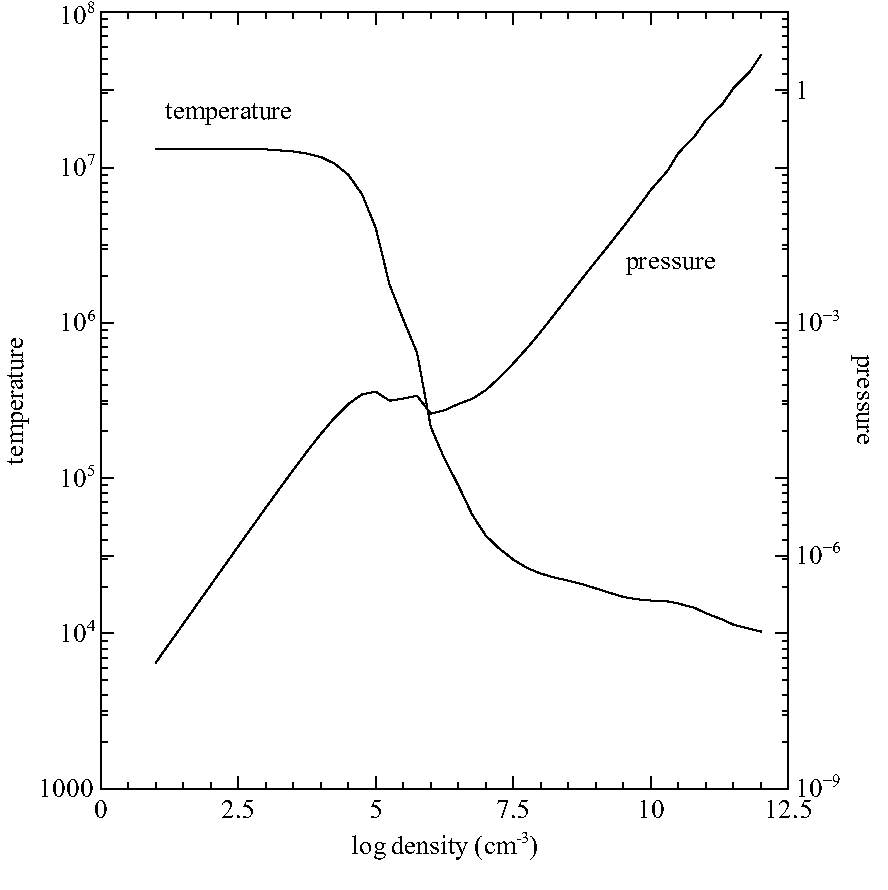
\includegraphics[scale=0.8]{hazy_kmt}
\caption[Temperature vs density in photoionization equilibrium]{\label{fig:hazy_kmt}Equilibrium temperature as a function of density.}
\end{figure}

\subsection{No Temperature Convergence}

A temperature failure occurs when the heating-cooling balance is not
within a certain tolerance,
set by the \cdCommand{set temperature error} command,
after 20 tries.
Normally \Cloudy\ will punt after an excessive number of temperature
failures occur.
The limit to the number of failures is reset with the
\cdCommand{failures} command.
If the \cdCommand{failures map} command is entered then the code
will first produce a map of heating-cooling space to give an indication
of where the equilibrium temperature should have been when excessive
failures occur.

Temperature failures most often occur for temperatures
in the range $10^2 \K$
to $4\times 10^3 \K$, and $10^5 \K$ to $10^6 \K$.
These are where the cooling function permits
more that one thermal solution (see, for example, \citealp{Williams1967}; \citealp{Dalgarno1972}).

Figure \ref{fig:cooling_heating} shows a typical cooling function for
gas in photoionization equilibrium.
A peak is reached at a temperature near $10^3 \K$.
This occurs
when the fine-structure lines are major coolants.
At lower temperatures
their cooling rate increases exponentially (as expected),
until roughly
$10^3 \K$, when their Boltzmann factors are near unity.
Above this temperature
their cooling rate is nearly proportional to the Coulomb focusing factor
$T^{-1/2}$, and the cooling \emph{decreases} until the temperature
is high enough for
optical forbidden lines to become important (at roughly $4000 \K$).
A similar
phenomenon occurs near the $\sim 10^5 \K$ to $10^6 \K$ peak in
the cooling function.

When failures occur because more than one temperature solution is
possible,  the reported failures are a physical (not numerical) problem.
\Cloudy\ will try to deal with this by forcing the temperature to
values below the peak in the cooling function.
Increasing the number of allowed failures
(with the \cdCommand{failures} command) to prevent the code from
stopping prematurely
is permissible as long as the global energy balance is preserved.
A warning
will be issued at the end of the calculation if the heating-cooling balance
is not preserved.

\subsection{Thermal Stability}

The thermal solution may be unstable when the temperature derivative
of the net cooling function (cooling minus heating) is negative (\citealp{Field1965}).
Possibly unstable solutions are indicated by a ``u'' just before the
equilibrium temperature in the zone printout.  The temperature derivative
is for isochoric (constant density), not isobaric (constant pressure),
conditions.  Comments are printed at the end of the calculation if possibly
unstable thermal solutions are present in the calculation.

\subsection{Thermal fronts}

Just as an ionization front is a region where the level of ionization
changes dramatically over a small scale, a thermal front occurs where the
temperature changes dramatically over a small scale.  This can be caused
by a real physical change of state of the gas such as those that occur near
the peaks in the cooling curve.
An example of a thermal front, taken from
\citet{FerlandFabian2002}, is shown in Figure \ref{fig:thermal_front}.
This type of jump is physical.
The gas changes phase and moves to different branches
of the cooling curve.
The code will generate a caution or comment if the
electron temperature changes discontinuously from one zone to the next.

\begin{figure}
\centering
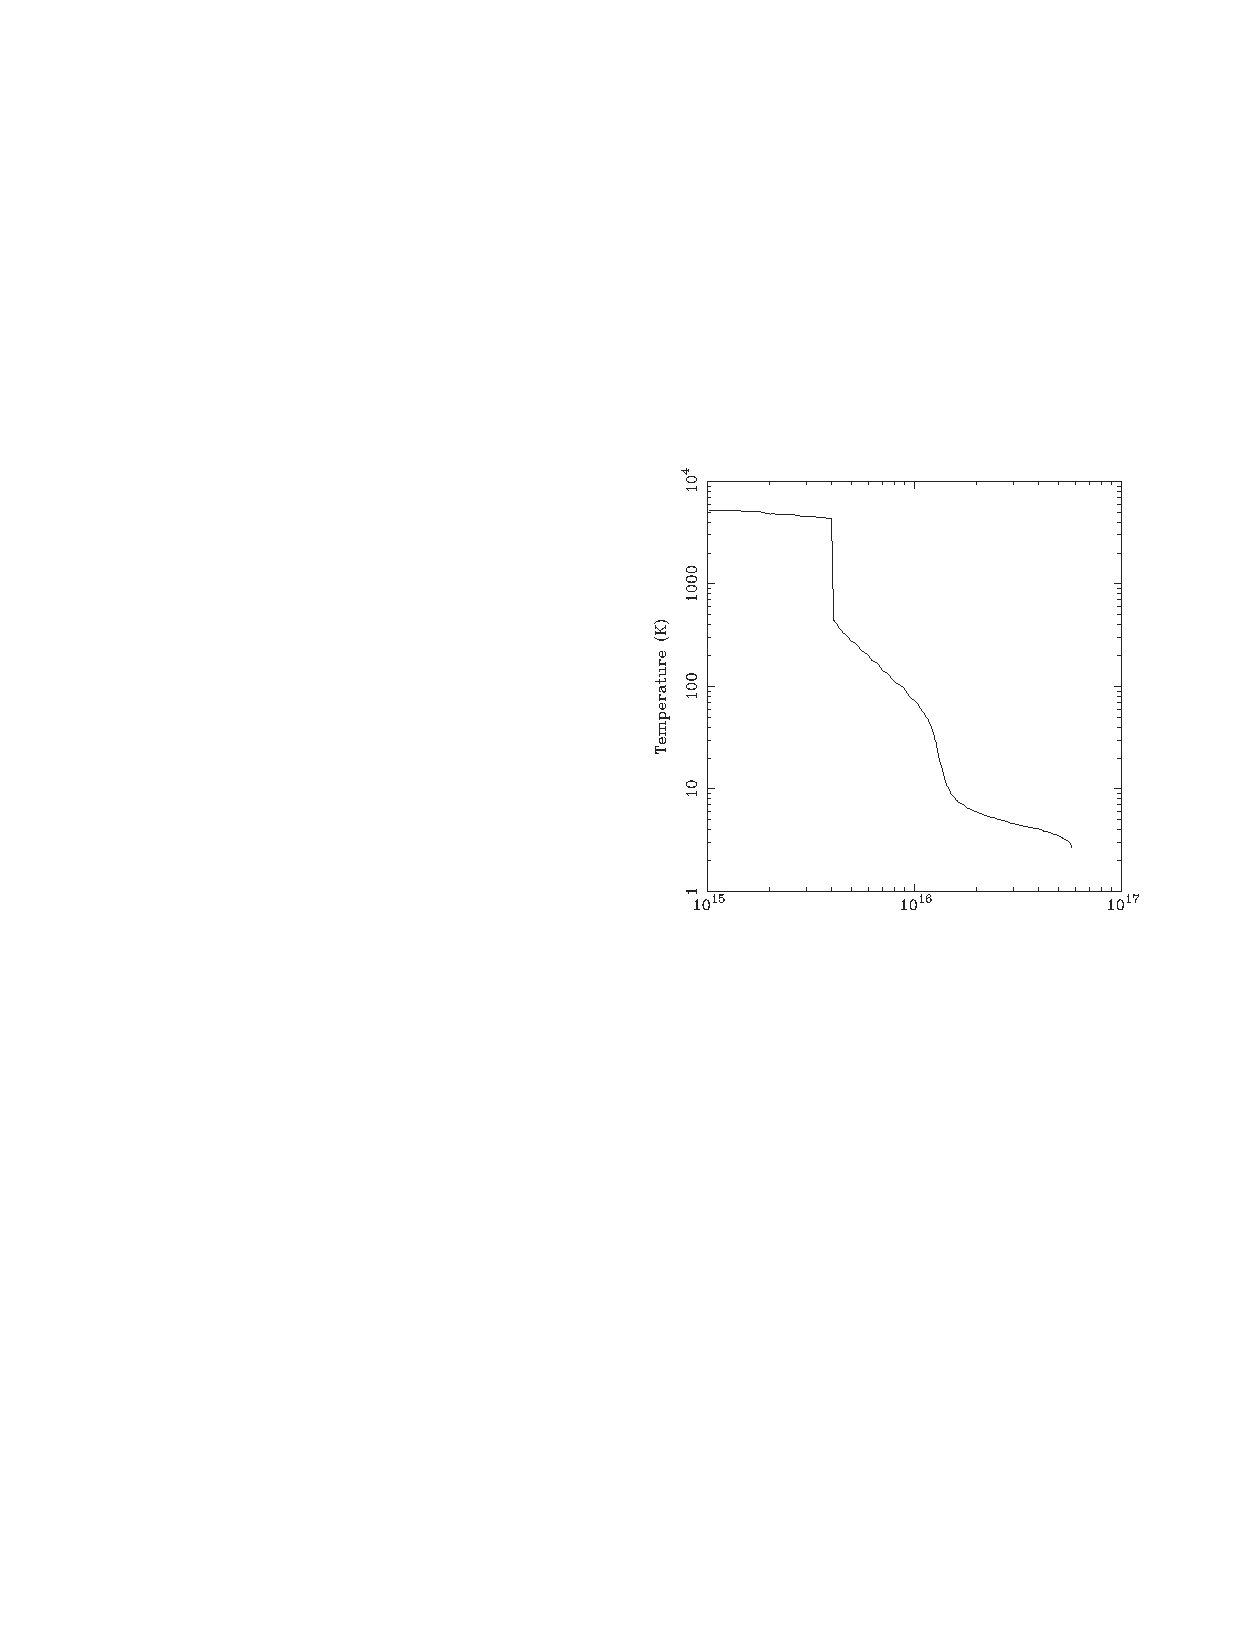
\includegraphics[scale=1.2]{thermal_front}
\caption[Thermal front example]{\label{fig:thermal_front}An example of a thermal front
in a cooling flow cloud
(\citealp{FerlandFabian2002}). The x-axis is the depth into the cloud (cm).
The thermal front at $\sim 4\times 10^{15}$~cm is unresolved.}
\end{figure}

A thermal front can lead to pressure convergence failures when the
solution jumps between the high and low temperature branches.
Figure \ref{fig:pressure_density}
shows an example case, taken from \cdFilename{orion\_hii\_pdr\_pp.in}
in the test suite.
This shows the pressure history (output with the
\cdCommand{save pressure history} command).
The solver adjusts the density trying to make the resulting
pressure agree with the desired pressure.
The pressure changes continuously
with density up to the point where the temperature jumps over the peak in
the cooling curve.
No solution is possible, and the code announces a
pressure failure.
In nature the presence of a magnetic field (added with
the \cdCommand{magnetic field} command) will cushion the front
from large changes in density.

\begin{figure}
\centering
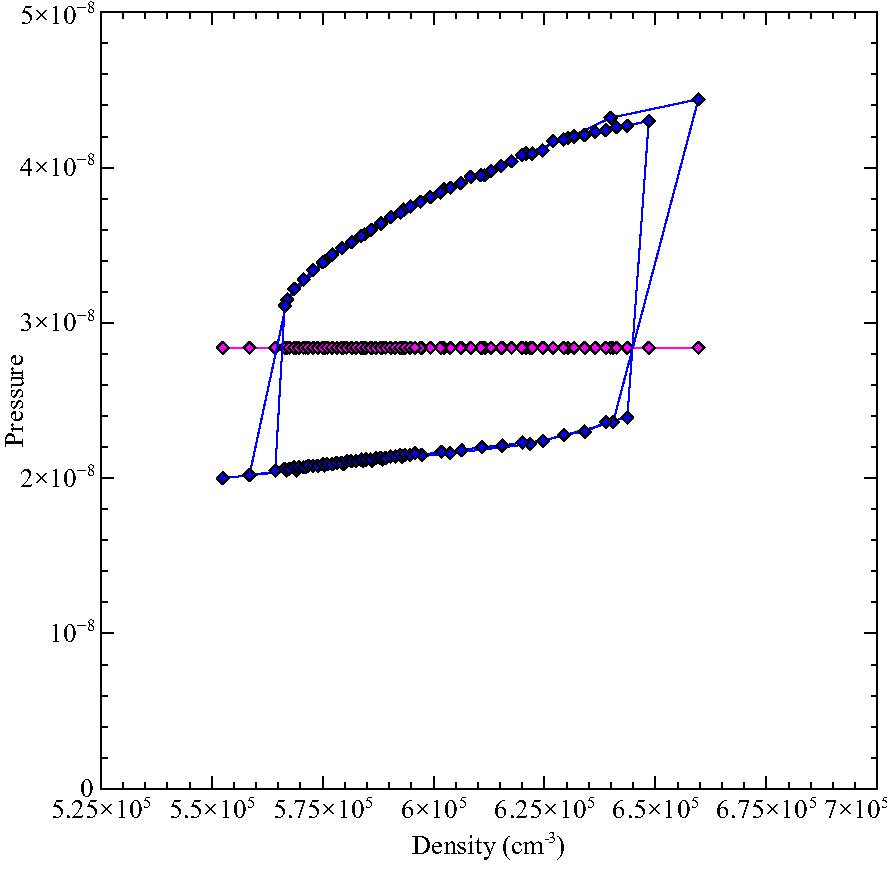
\includegraphics[scale=0.5]{pressure_density}
\caption[Thermal front]{\label{fig:pressure_density}A thermal front in a
constant pressure simulation.  The x-axis
gives the density [cm$^{-3}$] and the y-axis is the pressure
[dynes cm$^{-2}$].
The
points forming the large box are the resulting total gas pressure and the
horizontal line is the correct pressure.
The solution jumps above and below
the equilibrium value as the temperature jumps above and below the thermal
front.}
\end{figure}

A serious of pressure failures occur in this simulation when the gas
falls to a temperature of $\sim 300 \K$,
as shown in Figure \ref{fig:temperature_depth}.
The code simply
presses on with the goal of reaching the cold side of the front.

\begin{figure}
\centering
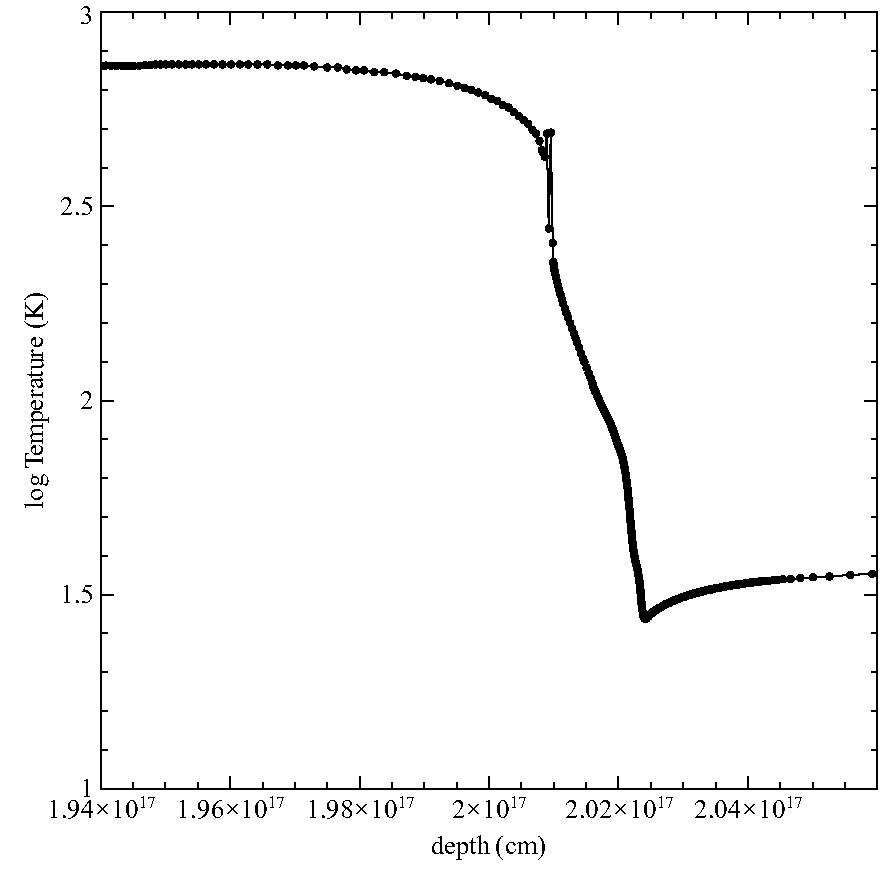
\includegraphics[scale=0.5]{temperature_depth}
\caption[Constant pressure thermal front]{\label{fig:temperature_depth}A constant-pressure thermal front
in a temperature - radius plot.
The x-axis gives the radius (cm).  The y-axis gives the log of the
temperature (K).
The solution jumps above and below the equilibrium value,
leading to a series of pressure failures, near a depth of
$2\times 10^{17}$~cm, as
it soldiers on through the thermal front.}
\end{figure}

\subsection{Map Output}

The program stops if an excessive number of temperature failures occur.
The default limit is 20.
It will produce a map of the heating and cooling
as a function of temperature for the last computed zone if the \cdCommand{map} option
on the \cdCommand{failures} command is given.
The map is described here.
The start
of the output from the test case \cdFilename{func\_map.in} is shown below.

\tiny
\begin{verbatim}
90.02x map of heating vs cooling
 te, heating, cooling.
 Cloudy punts, Te= 9.254E+03 HTOT= 9.123E-24 CTOT= 9.118E-24 nzone=   1
 COOLNG array is
     O  4    25  0.340 O  3  5007  0.182 O  3    88  0.075 H FB     0  0.057 S  4    10  0.048 O  3    51  0.042 S  3  9532 0.035
     H ff     0  0.022 S  3    33  0.020 Ne 3    15  0.019 Hefb     0  0.015 N  3    57  0.015 Ne 3  3869  0.013 S  3    18 0.013
     Ne 5    24  0.010 Ne 5    14  0.009 C  3  1910  0.008 Heff     0  0.007 Si 2    34  0.006 Fe 5  3892  0.006 O  2  3727 0.005
 Line heating array follows
    Te     Heat-------------------> Cool---------------------->    dH/dT    dC/DT       Ne         NH      HII       Helium
1.0000E+01 3.4774E-22   1   1 0.636 4.6095E-26 H FB    0A 0.723 -8.19E-24  1.56E-27 9.1178E-01 1.0000E+00 -0.07 -0.40 -0.24 -1.75
1.0209E+01 3.4490E-22   1   1 0.635 4.6814E-26 H FB    0A 0.720 -7.98E-24  1.65E-27 9.1353E-01 1.0000E+00 -0.07 -0.40 -0.23 -1.73
1.0423E+01 3.4233E-22   1   1 0.635 4.7510E-26 H FB    0A 0.717 -7.74E-24  1.74E-27 9.1491E-01 1.0000E+00 -0.07 -0.41 -0.23 -1.73
\end{verbatim}
\normalsize

The output begins with a listing of the strongest coolants for the last
zone.
Then the program steps through increasing temperatures and prints
the heating, cooling, and ionization of the gas.
From this information
it should be possible to determine the temperature where the equilibrium
thermal solution should have been.
Each solution is completely
self-consistent, except that heating and cooling do not balance.
Both the
local attenuated radiation field and collisional ionization contribute to
the ionization balance at each temperature.
All processes contribute to
the thermal balance, including collisional ionization.
The map is at
constant density.

The first column gives the temperature.
Columns 2 and 6 give the volume
heating and cooling.
Both have units erg s$^{-1}$ cm$^{-3}$.
Columns 3 and 4
constitute an indication of the main heating source.
Columns 7 and 8 give
the label and wavelength of the strongest coolant.
Columns 5 and 9 give
the fraction of the total heating or cooling due to these agents.
Columns
10 and 11 give the heating and cooling derivatives.
Columns 12 and 13 give
the electron and hydrogen densities (cm$^{-3}$) and the remaining columns give
the logs of the hydrogen and helium ionization fractions.
The location
of the probable thermal solution is indicated by a comment surrounded by
dashed lines.

\section{Convergence problems with dust-free static sphere}

Ionization convergence problems can occur with a dust-free static
spherical geometry.
The default geometry when the \cdCommand{sphere} command is entered
is for lines to freely escape after crossing the central hole due to some
level of expansion.
In a static spherical geometry (set with the
\cdCommand{sphere static} command) the total \la\ optical depth
at the illuminated face of the
shell will be very large since the line is scattered by the matter that
lies across the entire shell.
The line is destroyed when dust is present.
If dust is not present the \la\ intensity $J$ will become very large.  If the
total optical depth in \la\ is also large then the dominant escape /
destruction process for the line will be absorption by atoms of third-row
elements or the $n=2$ level of hydrogen.  This can lead to ionization
convergence problems due to the extremely large \la\ intensity $J$.

The first question to ask is whether this geometry is appropriate.  Dust
is nearly always present in the ISM.  In dense stellar environments it is
unlikely that a spherical geometry will be static.  Include dust, use the
default expanding spherical geometry, or a wind, and the problem will go
away.  To the best of my knowledge this geometry does not occur in nature.

\section{Optical depth convergence problems}

The code generally will not converge if it has not done so within ten
or so iterations.  Convergence problems most commonly occur when the
specified column density or thickness is very near a prominent ionization
front.  In this case very small changes in the physical conditions result
in large changes in the optical depths.
The code will not have convergence
problems if an optical depth is used as a stopping criterion instead.

\section{Negative populations}

It is possible that the code will stop because negative level populations
were predicted for atoms, ions, or molecules.
This is not supposed to occur,
but sometimes happens because of numerical instabilities in the matrix
inversion routine.
Please post the input stream and version of \Cloudy\ on
the code's discussion board.

\section{Floating Point Errors}

The code should be compiled and linked with options enabled so that the
code will crash on overflow or division by zero, but ignore underflow.
The \cdCommand{crash} command described in Part 1 tests this.  \emph{Floating point errors should never occur.}
The logic within the code is designed to identify
problems, and complain, but not fail.
The logic is only as good as the
tests they were designed to pass.
It is inevitable that circumstances will
occur for which the logic now in the code is not sufficient.
It is possible
that the code will fail when these circumstances occur.
I would be grateful
for reports of any such failures, since they inevitably identify shortcomings
in the code, and lead to its improvement.
Please post comments on the
discussion board on the code's web site.

\section{We can't fix it if we don't know it's broken}

Machines are growing faster far more rapidly than people are getting
smarter.
Reliability in the face of complexity is the major challenge to
the development of any large-scale computer code (\citealp{Ferland2001b}).  There
can be little doubt that \Cloudy\ contains bugs.

If problems arise or the code crashes then it is likely that you found
a problem.  We would appreciate learning about such problems since they
identify shortcomings which usually lead to improvements in the code (or
the documentation).  Please post queries and bug reports on the discussion
board on the code's discussion board.
